%review=doublespace preprint=single 5p=2 column
\documentclass[review]{elsarticle}

%% add packages %%
%% ------------ %%
\usepackage[hyphens]{url}
\usepackage{graphicx}
\usepackage{booktabs}
\usepackage[T1]{fontenc}
\usepackage{lmodern}
\usepackage{caption}
\usepackage{subfig}
\usepackage{amssymb, amsmath}
\usepackage[inline]{enumitem}
\usepackage{float}
\usepackage{tabularx}
\usepackage[dvipsnames, table]{xcolor}
\usepackage{ifxetex, ifluatex}
\usepackage{fixltx2e}
\usepackage[unicode=true, colorlinks]{hyperref}
\usepackage{cleveref}
%% ------------ %%

%% Conditional Packages %%
%% -------------------- %%



% use upquote if available, for straight quotes in verbatim environments
\IfFileExists{upquote.sty}{\usepackage{upquote}}{}

\ifnum 0\ifxetex 1\fi\ifluatex 1\fi=0 % if pdftex
  \usepackage[utf8]{inputenc}


\else % if luatex or xelatex
  \usepackage{fontspec}
  \ifxetex
    \usepackage{xltxtra,xunicode}
  \fi
  \defaultfontfeatures{Mapping=tex-text,Scale=MatchLowercase}
  \newcommand{\euro}{€}



    \setmonofont{sourcecodepro}


\fi

% use microtype if available
\IfFileExists{microtype.sty}{\usepackage{microtype}}{}






\usepackage{longtable}




% Pandoc toggle for numbering sections (defaults to be off)
\setcounter{secnumdepth}{5}

%% Use Landscape Pages


\usepackage{lmodern}

%% -------------------- %%

%% Create and Provide some customizations %%
%% -------------------------------------- %%
\providecommand{\tightlist}{%
  \setlength{\itemsep}{0pt}\setlength{\parskip}{0pt}}
  
%% Custom macros
\newtheorem{mydef}{Definition}
\newcommand{\bs}[1]{\ensuremath{\boldsymbol{#1}}}
\newcommand{\diag}[1]{\mathrm{diag}\left(#1\right)}
\newcommand{\seq}[3][1]{\ensuremath{#2_{#1},\ldots,\,#2_{#3}}}
\newcommand{\note}[1]{\marginpar{\scriptsize\tt{\color{RoyalBlue}#1}}}
\newcommand{\edit}[1]{{\color{OrangeRed} #1}}

% set some lengths
% \setlength{\parindent}{0pt}
% \setlength{\parskip}{6pt plus 2pt minus 1pt}
\setlength{\emergencystretch}{3em}  % prevent overfull lines

%% Hyperref color setup
\AtBeginDocument{%
  %% Define Colors
  \newcommand\myshade{80}
  \colorlet{mylinkcolor}{violet!\myshade!black}
  \colorlet{mycitecolor}{YellowOrange!\myshade!black}
  \colorlet{myurlcolor}{Aquamarine!\myshade!black}

  \hypersetup{
    breaklinks = true,
    bookmarks  = true,
    pdfauthor  = {},
    pdftitle   = {A tool for simulating multi-response linear model data},
    linkcolor  = mylinkcolor,
    citecolor  = mycitecolor,
    urlcolor   = myurlcolor,
    colorlinks = true,
  }
}
\urlstyle{same}  % don't use monospace font for urls
%% -------------------------------------- %%

%% Customizations %%
%% -------------- %%
 % turn line numbering on

%% -------------- %%

%% Configure Bibliography %%
%% ---------------------- %%
\bibliographystyle{elsarticle-harv}
\biboptions{square}

% \makeatletter
% \providecommand{\doi}[1]{%
%   \begingroup
%     \let\bibinfo\@secondoftwo
%     \urlstyle{rm}%
%     \href{http://dx.doi.org/#1}{%
%       doi:\discretionary{}{}{}%
%       \nolinkurl{#1}%
%     }%
%   \endgroup
% }
% \makeatother

% 

%% Header Includes %%
%% --------------- %%
%% --------------- %%



\usepackage{amsthm}
\newtheorem{theorem}{Theorem}[section]
\newtheorem{lemma}{Lemma}[section]
\theoremstyle{definition}
\newtheorem{definition}{Definition}[section]
\newtheorem{corollary}{Corollary}[section]
\newtheorem{proposition}{Proposition}[section]
\theoremstyle{definition}
\newtheorem{example}{Example}[section]
\theoremstyle{definition}
\newtheorem{exercise}{Exercise}[section]
\theoremstyle{remark}
\newtheorem*{remark}{Remark}
\newtheorem*{solution}{Solution}
\begin{document}
%% --- Front Matter Start --- %%
\begin{frontmatter}

  \title{A tool for simulating multi-response linear model data}
  
    \author[KBM]{Raju Rimal\corref{c1}}
   \ead{raju.rimal@nmbu.no} 
   \cortext[c1]{Corresponding Author}
    \author[KBM]{Trygve Almøy}
   \ead{trygve.almoy@nmbu.no} 
  
    \author[NMBU]{Solve Sæbø}
   \ead{solve.sabo@nmbu.no} 
  
      \address[KBM]{Faculty of Chemistry and Bioinformatics, Norwegian University of Life
Sciences, Ås, Norway}
    \address[NMBU]{Prorector, Norwegian University of Life Sciences, Ås, Norway}
  
  \begin{abstract}
  Data science is generating enormous amounts of data, and new and
  advanced analytical methods are constantly being developed to cope with
  the challenge of extracting information from such ``big-data''.
  Researchers often use simulated data to assess and document the
  properties of these new methods, and in this paper we present an
  extension to the R-package \texttt{simrel}, which is a versatile and
  transparent tool for simulating linear model data with an extensive
  range of adjustable properties. The method is based on the concept of
  relevant components \citep{helland1994comparison}, and is equivalent to
  the envelope model by Dennis Cook. It is a multi-response extension of
  R-package \texttt{simrel} which is available in R-package repository
  CRAN, and as \texttt{simrel} the new approach is essentially based on
  random rotations of latent relevant components to obtain a predictor
  matrix \(\mathbf{X}\), but in addition we introduce random rotations of
  latent components spanning a response space in order to obtain a
  multivariate response matrix \(\mathbf{Y}\). The properties of the
  linear relation between \(\mathbf{X}\) and \(\mathbf{Y}\) are defined by
  a small set of input parameters which allow versatile and adjustable
  simulations. Sub-space rotations also allow for generating data suitable
  for testing variable selection methods in multi-response settings. The
  method is implemented as an update to the R-package \texttt{simrel}.
  \end{abstract}
   \begin{keyword} \texttt{simrel} package in r,data simulation,linear model\end{keyword}

\end{frontmatter}

\section{Introduction}\label{introduction}

Technological advancement has opened a door for complex and
sophisticated scientific experiments that was not possible before. Due
to this change, enormous amounts of raw data are generated which contain
massive information but is difficult to excavate. Finding information
and performing scientific research on these raw data has now become
another problem. In order to tackle this situation new methods are being
developed. However, before implementing any method, it is essential to
test its performance and explore its properties. Often, researchers use
simulated data for the purpose which itself is a time-consuming process.
The main focus of this paper is to present a simulation method, along
with an extension to the r-package called \texttt{simrel}, that is
versatile in nature and yet simple to use.

The simulation method we are presenting here is based on the principle
of relevant space for prediction \citep{helland1994comparison} which
assumes that there exists a y-relevant subspace in the complete space of
predictor variables that is spanned by a subset of eigenvectors of these
predictor variables. Our extension to this principle is to introduce a
subspace in \(\mathbf{y}\) (material space) which contains the
information that predictor space is relevant for. The concept of
response reduction to the material space in response variable was
introduced by \citet{cook2010envelope}. Our r-package based on this
principle lets the user to specify various population properties such
as, which latent components are relevant for a latent subspace of the
responses \(\mathbf{y}\) and the collinearity structure of
\(\mathbf{x}\). This enables the possibility to construct data for
evaluating estimation methods and methods developed for variable
selection.

Among several publications on simulation, \citet{ripley2009stochastic}
and \citet{gamerman2006markov} have exhaustively discussed the topic. In
addition, many publications have implemented simulated data in order to
investigate new estimation methods and prediction strategies
\citep[see:][]{cook2015simultaneous, cook2013envelopes, helland2012near}.
However, most of the simulations in these studies were developed to
address their specific problem. A systematic tool for simulating linear
model data with single response, which could serve as a general tool for
all such comparisons, was presented in \citet{saebo2015simrel} and as
the r-package \texttt{simrel}. This paper extends \texttt{simrel} in
order to simulate linear model data with multivariate response.

\section{Statistical Model}\label{statistical-model}

In this section we describe the model and the model parameterization
which is assumed throughout this paper. We assume:

\begin{equation}
  \begin{bmatrix}\mathbf{y}\\ \mathbf{x}\end{bmatrix} \sim N
  \left(
    \begin{bmatrix}
      \boldsymbol{\mu}_y \\
      \boldsymbol{\mu}_x
    \end{bmatrix},
    \begin{bmatrix}
      \boldsymbol{\Sigma}_{yy} & \boldsymbol{\Sigma}_{yx} \\
      \boldsymbol{\Sigma}_{yx}^t & \boldsymbol{\Sigma}_{xx}
    \end{bmatrix}
  \right)
  \label{eq:rand-reg-model}
\end{equation}

where, \(\mathbf{y}\) is a response vector with \(m\) response variables
\(y_1, y_2, \ldots y_m\) with mean vector \(\boldsymbol{\mu}_y\), and
\(\mathbf{x}\) is vector of \(p\) predictor variables with mean vector
\(\boldsymbol{\mu}_x\). Further,

\begin{longtable}[]{@{}ll@{}}
\toprule
\(\boldsymbol{\Sigma}_{yy} (m \times m)\) & is the variance-covariance
matrix of \(\mathbf{y}\)\tabularnewline
\(\boldsymbol{\Sigma}_{xx} (p \times p)\) & is the variance-covariance
matrix of variables \(\mathbf{x}\)\tabularnewline
\(\boldsymbol{\Sigma}_{yx} (m \times p)\) & is the matrix of covariance
between \(\mathbf{x}\) and \(\mathbf{y}\)\tabularnewline
\bottomrule
\end{longtable}

\addtocounter{table}{-1}

Standard theory in multivariate statistics may be used to show that
\(\mathbf{y}\) conditioned on \(\mathbf{x}\) corresponds to the linear
model,

\begin{equation}
\mathbf{y} = \boldsymbol{\mu}_y + \boldsymbol{\beta}^t (\mathbf{x} - \boldsymbol{\mu}_x) + \boldsymbol{\varepsilon}
  \label{eq:linear-model}
\end{equation}

where, \(\boldsymbol{\beta}^t\) is a \((m \times p)\) matrix of
regression coefficient, and \(\boldsymbol{\varepsilon}\) is an error
term such that
\(\boldsymbol{\varepsilon} \sim N\left(0, \boldsymbol{\Sigma}_{y|x}\right)\).
The properties of the linear model \eqref{eq:linear-model} can be
expressed in terms of covariance matrices in \eqref{eq:rand-reg-model}.

\begin{description}
\tightlist
\item[Regression Coefficients]
The matrix of regression coefficients is given by
\[ \boldsymbol{\beta} = \boldsymbol{\Sigma}_{xx}^{-1}\boldsymbol{\Sigma}_{xy}\]
\item[Coefficient of Determination]
The diagonal elements of the coefficient-of-determination matrix
\(\boldsymbol{\rho}_y^2 (m \times m)\) gives the amount of variation in
each response variable that is explained by \(\mathbf{x}\).
\[\boldsymbol{\rho}_y^2 = \boldsymbol{\Sigma}_{yx}\boldsymbol{\Sigma}_{xx}^{-1}\boldsymbol{\Sigma}_{xy}\boldsymbol{\Sigma}_{yy}^{-1}\]
\item[Conditional variance]
The conditional variance-covariance matrix of \(\mathbf{y}\) given
\(\mathbf{x}\) is,
\[\boldsymbol{\Sigma}_{y|x} = \boldsymbol{\Sigma}_{yy} - \boldsymbol{\Sigma}_{yx}\boldsymbol{\Sigma}_{xx}^{-1}\boldsymbol{\Sigma}_{xy}.\]
The diagonal elements of this matrix equals the minimum least square
error of prediction \(\left[\mathrm{E}(y - \hat{y})^2\right]\) for each
of the response variables.
\end{description}

Let us define a transformation of \(\mathbf{x}\) and \(\mathbf{y}\) as,
\(\mathbf{z} = \mathbf{Rx}\) and \(\mathbf{w} = \mathbf{Qy}\). Here,
\(\mathbf{R}_{p\times p}\) and \(\mathbf{Q}_{m\times m}\) are rotation
matrices that rotate \(\mathbf{x}\) and \(\mathbf{y}\) to yield
\(\mathbf{z}\) and \(\mathbf{w}\), respectively. The model
\eqref{eq:rand-reg-model} can be re-expressed in terms of these
transformed variables as:

\begin{align}
  \begin{bmatrix}\mathbf{w} \\ 
  \mathbf{z}\end{bmatrix}  & \sim N \left(\boldsymbol{\mu}, \boldsymbol{\Sigma}\right)
  = N \left(
    \begin{bmatrix}
      \boldsymbol{\mu}_w \\ \boldsymbol{\mu}_z
    \end{bmatrix},
    \begin{bmatrix}
      \boldsymbol{\Sigma}_{ww} & \boldsymbol{\Sigma}_{wz} \\
      \boldsymbol{\Sigma}_{zw} & \boldsymbol{\Sigma}_{zz}
    \end{bmatrix} \right) \nonumber \\
  &= N \left(
    \begin{bmatrix}
      \boldsymbol{Q\mu}_y \\
      \boldsymbol{R\mu}_x
    \end{bmatrix},
    \begin{bmatrix}
      \boldsymbol{Q\Sigma}_{yy}\boldsymbol{Q}^t & \boldsymbol{Q\Sigma}_{yx}\mathbf{R}^t \\
      \boldsymbol{R\Sigma}_{xy}\boldsymbol{Q}^t & \boldsymbol{R\Sigma}_{xx}\mathbf{R}^t
    \end{bmatrix}
  \right)
  \label{eq:model3}
\end{align}

In addition, a linear model relating \(\mathbf{w}\) conditioned on
\(\mathbf{z}\) can be written as,

\begin{equation}
\mathbf{w} =    \boldsymbol{\mu}_w + \boldsymbol{\alpha}^t \left(\mathbf{z} - \boldsymbol{\mu}_z\right) + \boldsymbol{\tau}
\label{eq:latent-model}
\end{equation}

where \(\boldsymbol{\alpha}\) is the regression coefficient vector for
the transformed model and
\(\boldsymbol{\tau} \sim N\left(\mathbf{0}, \boldsymbol{\Sigma}_{w|z}\right)\).
Further, if both \(\mathbf{Q}\) and \(\mathbf{R}\) are orthonormal
matrices, i.e., \(\mathbf{Q}^t\mathbf{Q} = \mathbf{I}_q\) and
\(\mathbf{R}^t\mathbf{R} = \mathbf{I}_p\), the inverse transformation
can be defined as,

\begin{equation}
  \begin{matrix}
    \boldsymbol{\Sigma}_{yy} = \mathbf{Q}^t \boldsymbol{\Sigma}_{ww} \mathbf{Q} &
    \boldsymbol{\Sigma}_{yx} = \mathbf{Q}^t \boldsymbol{\Sigma}_{wz} \mathbf{R} \\
    \boldsymbol{\Sigma}_{xy} = \mathbf{R}^t \boldsymbol{\Sigma}_{zw} \mathbf{Q} &
    \boldsymbol{\Sigma}_{xx} = \mathbf{R}^t \boldsymbol{\Sigma}_{zz} \mathbf{R}
  \end{matrix}
  \label{eq:cov-yx-wz}
\end{equation}

From this, we can find a direct connection between different population
properties of \eqref{eq:linear-model} and \eqref{eq:latent-model}.

\begin{description}
\tightlist
\item[Regression Coefficients]
\[
  \begin{aligned}
  \boldsymbol{\alpha} &= \boldsymbol{\Sigma}_{wz} \boldsymbol{\Sigma}_{zz}^{-1}
  = \boldsymbol{Q\Sigma}_{yz}\mathbf{R}^t\left[\boldsymbol{R\Sigma}_{xx}\mathbf{R}^t\right]^{-1}
  = \mathbf{Q}\left[\boldsymbol{\Sigma}_{yx}\boldsymbol{\Sigma}_{xx}^{-1}\right]\mathbf{R}^t
  = \mathbf{Q}\boldsymbol{\beta}\mathbf{R}^t
  \end{aligned}
  \]
\item[Conditional Variance]
Further, the conditional variance-covariance matrix of \(\mathbf{w}\)
given \(\mathbf{z}\) is, \[
  \begin{aligned}
\boldsymbol{\Sigma}_{w|z}
&= \boldsymbol{\Sigma}_{ww} - \boldsymbol{\Sigma}_{wz}\boldsymbol{\Sigma}_{zz}^{-1}\boldsymbol{\Sigma}_{zw} \\
&= \boldsymbol{Q\Sigma}_{yy}\mathbf{Q}^t -
  \boldsymbol{Q \Sigma}_{yx}\mathbf{R}^t \left[\boldsymbol{R\Sigma}_{xx}\boldsymbol{R}^t\right]^{-1}
  \boldsymbol{R\Sigma}_{xy}\mathbf{Q}^t \nonumber \\
&= \boldsymbol{Q\Sigma}_{yy}\mathbf{Q}^t - 
  \boldsymbol{Q \Sigma}_{yx}\boldsymbol{\Sigma}_{xx}^{-1}\boldsymbol{\Sigma}_{xy}\mathbf{Q}^t \\
&= \mathbf{Q}\left[\boldsymbol{\Sigma}_{yy} -
  \boldsymbol{\Sigma}_{yx}\boldsymbol{\Sigma}_{xx}^{-1}\boldsymbol{\Sigma}_{xy}\right]\mathbf{Q}^{t}
= \mathbf{Q} \boldsymbol{\Sigma}_{y|x}\mathbf{Q}^t
  \end{aligned}
  \]
\item[Coefficient of Determination]
The coefficient-of-determination matrix for \eqref{eq:latent-model} is, \[
  \begin{aligned}
\boldsymbol{\rho}^2_w &= \boldsymbol{\Sigma}_{wz} 
\boldsymbol{\Sigma}_{zz}^{-1} \boldsymbol{\Sigma}_{zw} 
\boldsymbol{\Sigma}_{ww}^{-1} \\
  &=\mathbf{Q}^t
  \boldsymbol{\Sigma}_{yx}\mathbf{R}^t \left(\mathbf{R}\boldsymbol{\Sigma}_{xx}\mathbf{R}^t\right)^{-1}
  \mathbf{R}\boldsymbol{\Sigma}_{xy}\mathbf{Q}^t \left(\mathbf{Q} \boldsymbol{\Sigma}_{yy}^{-1} \mathbf{Q}^t\right) \nonumber \\
  &=\mathbf{Q}^t\left[\boldsymbol{\Sigma}_{yx}\boldsymbol{\Sigma}_{xx}\boldsymbol{\Sigma}_{xy}\boldsymbol{\Sigma}_{yy}^{-1}\right]\mathbf{Q}
  = \mathbf{Q}\boldsymbol{\rho}_{Y}^2 \mathbf{Q}^t
  \end{aligned}
  \]
\end{description}

From the eigenvalue decomposition principle, if
\(\boldsymbol{\Sigma}_{xx} = \mathbf{R}\boldsymbol{\Lambda}\mathbf{R}^t\)
and
\(\boldsymbol{\Sigma}_{yy} = \mathbf{Q}\boldsymbol{\Omega}\mathbf{Q}^t\)
then \(\mathbf{z}\) and \(\mathbf{w}\) can be interpreted as principal
components of \(\mathbf{x}\) and \(\mathbf{y}\) respectively. In this
paper, these principal components will be termed as \emph{predictor
components} and \emph{response components} respectively. Here,
\(\boldsymbol{\Lambda}\) and \(\boldsymbol{\Omega}\) are diagonal
matrices of eigenvalues of \(\boldsymbol{\Sigma}_{xx}\) and
\(\boldsymbol{\Sigma}_{yy}\), respectively.

\section{Relevant Components}\label{relevant-components}

Consider a single response linear model with \(p\) predictors.

\[y = \mu_y + \boldsymbol{\beta}^t\left(\mathbf{x} - \mu_x\right) + \epsilon\]

where, \(\epsilon \sim N(0, \sigma^2)\) and \(\mathbf{x}\) is a vector
of random predictors. Following the concept of relevant space and
irrelevant space which is discussed extensively in
\citet{helland1994comparison}, \citet{Helland2000},
\citet{helland2012near}, \citet{cook2013envelopes}, and
\citet{saebo2015simrel}, we can assume that there exists a subspace of
the full predictor space which is relevant for \(y\). An orthogonal
space to this space does not contain any information about \(y\) and is
considered as irrelevant. Here, the \(y-\)relevant subspace of
\(\mathbf{x}\) is spanned by a subset of the principal components
defined by the eigenvectors of the covariance matrix of \(\mathbf{x}\),
i.e. \(\boldsymbol{\Sigma}_{xx}\).

This concept can be extended to \(m\) responses so that the subspace of
\(\mathbf{x}\) is relevant for a subspace of \(\mathbf{y}\). This
corresponds to the concept of simultaneous envelopes
\citep{cook2015simultaneous} where relevant (material) and irrelevant
(immaterial) space were discussed for both response and predictor
variables.

\subsection{Model Parameterization}\label{model-parameterization}

In order to construct a fully specified and unrestricted covariance
matrix of \(\mathbf{z}\) and \(\mathbf{w}\) for the model in equation
\eqref{eq:model3}, we need to identify \(1/2 (p+m)(p+m+1)\) unknown
parameters. For the purpose of simulation, we implement some assumptions
to re-parameterize and simplify the model. This enables us to construct
a wide range of model properties from only few key parameters.

\begin{description}
\tightlist
\item[\textbf{Parameterization of \(\boldsymbol{\Sigma}_{zz}\)}]
If we let the rotation matrix \(\mathbf{R}\) correspond to the
eigenvectors of \(\boldsymbol{\Sigma}_{xx}\), then \(\mathbf{z}\)
becomes the set of principal components of \(\mathbf{x}\). In that case
\(\boldsymbol{\Sigma}_{zz}\) is a diagonal matrix with eigenvalues
\(\lambda_1, \ldots, \lambda_p\). Further, we adopt the same parametric
representation as \citet{saebo2015simrel} for these eigenvalues:
\[\lambda_j = e^{-\gamma(j - 1)}, \gamma >0 \text{ and } j = 1, 2, \ldots, p\]
Here, as \(\gamma\) increases, the decline of eigenvalues becomes
steeper, hence the parameter \(\gamma\) controls the level of
multicollinearity in \(\mathbf{x}\).
\item[\textbf{Parameterization of \(\boldsymbol{\Sigma}_{ww}\)}]
Here we assume that \(\mathbf{w}\)'s are independent and has mutinormal
distribution with variances 1, hence
\(\boldsymbol{\Sigma}_{ww} = \mathbf{I}_m\).
\item[\textbf{Parameterization of \(\boldsymbol{\Sigma}_{zw}\)}]
After parameterization of \(\boldsymbol{\Sigma}_{zz}\) and
\(\boldsymbol{\Sigma}_{ww}\), we are left with \(m \times p\) number of
unknowns corresponding to \(\boldsymbol{\Sigma}_{zw}\). Some of the
elements of \(\boldsymbol{\Sigma}_{zw}\) may be equal to zero, which
implies that the given \(z\) is irrelevant for the given variable \(w\).
The non-zero elements define which of the \(z\) are relevant for
\(\mathbf{w}\). We typically refer to the indices of these \(z\)
variables as the positions of relevant components. In order to
re-parameterize this covariance matrix, it is necessary to discuss the
position of relevant components in detail.
\end{description}

\subsubsection{Position of relevant
components}\label{position-of-relevant-components}

Let \(k_1\) components be relevant for \(w_1\), \(k_2\) components be
relevant for \(w_2\) and so on. Let the positions of these components be
given by the index sets
\(\mathcal{P}_1, \mathcal{P}_2, \ldots, \mathcal{P}_m\) respectively.
Further, the covariance between \(w_j\) and \(z_i\) is non-zero only if
\(z_i\) is relevant for \(w_j\). If \(\sigma_{ij}\) is the covariance
between \(w_j\) and \(z_i\) then \(\sigma_{ij} \ne 0\) if
\(i \in \mathcal{P}_j\) where \(i = 1, \ldots, p\) and
\(j = 1, \ldots, m\) and \(\sigma_{ij} = 0\) otherwise.

In addition, the true regression coefficients for \(w_j\)
{[}ref:\eqref{eq:latent-model}{]} is given by:

\[
\boldsymbol{\alpha}_j = \Lambda^{-1} \sigma_{ij} = \sum_{i \in \mathcal{P}_j}\frac{\sigma_{ij}}{\lambda_i},\qquad j = 1, 2, \ldots m
\]

The positions of the relevant components have heavy impact on
prediction. \citet{helland1994comparison} have shown that if the
relevant components have large eigenvalues (variances), which here
implies small index values in \(\mathcal{P}_j\), prediction of
\(\mathbf{y}\) from \(\mathbf{x}\) is relatively easy and if the
eigenvalues (variances) of relevant components are small, the prediction
becomes difficult, given that the coefficient of determination and other
model parameters are held constant. For example, if the first and second
components, \(z_1\) and \(z_2\), are relevant for \(w_1\) and fifth and
sixth components, \(z_5\) and \(z_6\), are relevant for \(w_2\), it is
relatively easier to predict \(w_1\) than \(w_2\), other properties
being similar. This might be so, because the first and second principal
components have larger variances than the fifth and sixth components.

Although the covariance matrix may depend on few relevant components, we
can not choose these covariances freely since we also need to satisfy
following two conditions:

\begin{itemize}
\tightlist
\item
  The covariance matrices \(\Sigma_{zz}\), \(\Sigma_{ww}\) and
  \(\Sigma\) must be positive definite
\item
  The covariance \(\sigma_{ij}\) must satisfy user defined coefficient
  of determination
\end{itemize}

We have the relation,
\[\boldsymbol{\rho}_w^2 = \boldsymbol{\Sigma}_{zw}^t\boldsymbol{\Sigma}_{zz}^{-1}\boldsymbol{\Sigma}_{zw}\boldsymbol{\Sigma}_{ww}^{-1}\]
Applying our assumptions that,
\(\boldsymbol{\Sigma_{ww}} = \mathbf{I}_m\) and
\(\boldsymbol{\Sigma}_{zz} = \Lambda\), we obtain,

\[
\begin{aligned}
\boldsymbol{\rho}_w^2 &= \boldsymbol{\Sigma}_{zw}^t \Lambda^{-1} \boldsymbol{\Sigma}_{zw} \mathbf{I}_m \\
&= \begin{bmatrix}
\sum_{i = 1}^p \sigma_{i1}^2/\lambda_i          & \ldots & \sum_{i = 1}^p \sigma_{i1}\sigma_{im}/\lambda_i \\
\vdots                                          & \ddots & \vdots \\
\sum_{i = 1}^p \sigma_{i1}\sigma_{im}/\lambda_i & \ldots & \sum_{i = 1}^p \sigma_{im}^2/\lambda_i
\end{bmatrix}
\end{aligned}
\]

Furthermore, we assume that there are no overlapping relevant components
for any two \(w\), i.e,
\(\mathcal{P}_j \cap \mathcal{P}_{j*} = \varnothing\) or
\(\sigma_{ij}\sigma_{ij*} = 0\) for \(j\ne j*\). The additional unknown
parameters in the diagonal of \(\boldsymbol{\rho}_w^2\) should agree
with user specified coefficients of determination for \(\mathbf{w}\).
i.e, \(\rho_{wj}^2\) is,

\[
\rho_{wj}^2 = \sum_{i = 1}^p\frac{\sigma_{ij}^2}{\lambda_i}
\]

Here, only the relevant components have non-zero covariances with
\(w_j\), so,

\[
\rho_{wj}^2 = \sum_{i \in \mathcal{P}_j}\frac{\sigma_{ij}^2}{\lambda_i}
\]

For some user defined \(\rho_{jw}^2\) the \(\sigma_{ij}^2\) is
determined as follows,

\begin{enumerate}
\def\labelenumi{\arabic{enumi}.}
\tightlist
\item
  Sample \(k_j\) values from a uniform distribution
  \(\mathcal{U}(-1, 1)\) distribution. Let them be denoted
  \(\mathcal{S}_{\mathcal{P}_1}, \ldots, \mathcal{S}_{\mathcal{P}_{k_j}}\).
\item
  Define,
  \[\sigma_{ij} = \text{Sign}\left(\mathcal{S}_i\right)\sqrt{\frac{\rho_{wj}^2\left|\mathcal{S}_i\right|}{\sum_{k\in \mathcal{P}_j}\left|\mathcal{S}_k\right|} \lambda_i}\]
  for \(i \in \mathcal{P}_j\) and \(j = 1, \ldots, m\)
\end{enumerate}

\subsubsection{Data Simulation}\label{data-simulation}

From the above given parameterizations and the user defined choices of
model parameters, a fully defined and known covariance matrix
\(\boldsymbol{\Sigma}\) of \((\mathbf{w, z})\) is given. For the
simulation of a single observation of \((\mathbf{w, z})\) let us define
\(\mathbf{g} = \boldsymbol{\Sigma}^{-1/2}\mathbf{u}\) such that
\(\text{cov}(\mathbf{g}) = \boldsymbol{\Sigma}\). Here
\(\boldsymbol{\Sigma}^{-1/2}\) is obtained from Choleskey decomposition
of \(\boldsymbol{\Sigma}\), and \(\mathbf{u}\) is simulated from
independent standard normal distribution.

Similarly, in order to simulate \(n\) observations, we define
\(\underset{n \times (m + p)}{\mathbf{G}} = \mathbf{U}\boldsymbol{\Sigma}^{-1/2}\).
Here the first \(m\) columns of \(\mathbf{G}\) will serve as
\(\mathbf{W}\) and remaining \(p\) columns will serve as \(\mathbf{Z}\).
Further, each row of \(\mathbf{G}\) will be a vector sampled
independently from the joint normal distribution of
\(\left(\mathbf{w}, \mathbf{z}\right)\). Finally, these simulated
matrices \(\mathbf{W}\) and \(\mathbf{Z}\) are orthogonally rotated in
order to obtain \(\mathbf{Y}\) and \(\mathbf{X}\) respectively. The
following section discuss about these rotation matrices in detail.

\subsection{Rotation of predictor
space}\label{rotation-of-predictor-space}

Initially, let us consider an example where a regression model with
\(p = 10\) predictors \((\mathbf{x})\) and \(m = 4\) responses
\((\mathbf{y})\). Let's assume that only three response components
\((w_1, w_2\) and \(w_3)\) are needed to describe all four response
variables. Further, let the index sets
\(\mathcal{P}_1 = \{1, 2\}, \mathcal{P}_2 = \{3, 4\}\) and
\(\mathcal{P}_3 = \{5, 6\}\) define the positions of the predictor
components of \(\mathbf{x}\) that are relevant for \(w_1, w_2\) and
\(w_3\) respectively. Let \(\mathcal{S}_1\), \(\mathcal{S}_2\) and
\(\mathcal{S}_3\) be the orthogonal spaces spanned by each set of
predictor components. These spaces together span
\(\mathcal{S}_k = \mathcal{S}_1 \oplus \mathcal{S}_2 \oplus \mathcal{S}_3\)
which is the minimum relevant space and equivalent to the x-envelope as
discussed by \citet{cook2013envelopes}.

Moreover, let \(q_1 = 3, q_2 = 3\) and \(q_3 = 2\) be the number of
predictor variables we want to have relevant for \(w_1, w_2\) and
\(w_3\) respectively. Then \(q_1 = 3\) predictors may be obtained by
rotating the predictor components in \(\mathcal{P}_1\) along with one
more irrelevant component. Similarly, \(q_2 = 3\) predictors, relevant
for \(w_2\), can be obtained by rotating predictor components in
\(\mathcal{P}_2\) along with one more irrelevant component and finally,
\(q_3 = 2\) predictors, relevant for \(w_3\), can be obtained by
rotating the components in \(\mathcal{P}_3\) without any additional
irrelevant component. Let the space spanned by the \(q_1, q_2\) and
\(q_3\) number of predictors be \(\mathcal{S}_{q_1}\),
\(\mathcal{S}_{q_2}\) and \(\mathcal{S}_{q_3}\). Together they span a
space
\(\mathcal{S}_q = \mathcal{S}_{q_1} \oplus \mathcal{S}_{q_2} \oplus \mathcal{S}_{q_3}\).
This space is bigger than \(\mathcal{S}_k\) since in the process two
irrelevant components were included in the rotations. Here,
\(\mathcal{S}_k\) is orthogonal to \(\mathcal{S}_{p - k}\) and
\(\mathcal{S}_q\) is orthogonal to \(\mathcal{S}_{p - q}\). Generally
speaking, here we are splitting the complete variable space
\(\mathcal{S}_p\) into two orthogonal spaces -- \(\mathcal{S}_k\)
relevant for \(\mathbf{w}\) and \(\mathcal{S}_{p - k}\) irrelevant for
\(\mathbf{w}\).

In the previous section, we discussed about the construction of a
covariance matrix for the latent structure. Figure
\ref{fig:cov-plot-print}(a) shows a similar structure resembling the
example here. The three colors represent the relevance with the three
latent response components \((w_1, w_2\) and \(w_3)\). Here we can see
that \(z_{1}\) and \(z_{2}\) (first and second predictor components of
\(\mathbf{x}\)) have non-zero covariance with \(w_1\) (first latent
component of response \(\mathbf{y}\)). In the similar manner other
non-zero covariances are self-explanatory.

\begin{figure}[!htb]
\subfloat[Relevant Position\label{fig:cov-plot-print1}]{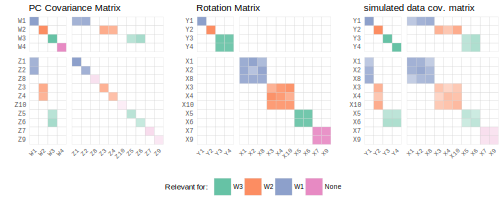
\includegraphics[width=0.33\linewidth]{main_files/figure-latex/cov-plot-print-1} }\subfloat[Rotation Matrix\label{fig:cov-plot-print2}]{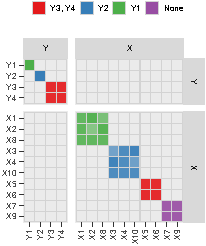
\includegraphics[width=0.33\linewidth]{main_files/figure-latex/cov-plot-print-2} }\subfloat[Relevant Predictors\label{fig:cov-plot-print3}]{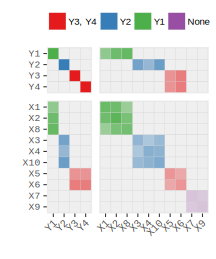
\includegraphics[width=0.33\linewidth]{main_files/figure-latex/cov-plot-print-3} }\caption{Simulation of predictor and response variables after orthogonal transformation of predictor and response components by rotation matrices $Q$ and $R$ shown as the upper left and the lower right block matrices in (b).}\label{fig:cov-plot-print}
\end{figure}

In order to simulate predictor variables \((\mathbf{x})\), we construct
matrix \(\mathbf{R}\) which then is used for orthogonal rotation of the
predictor components \(\mathbf{z}\). This defines a new basis for the
same space as is spanned by the predictor components. In principle,
there are many possible options for defining a rotation matrix. Among
them, the eigenvector matrix of \(\boldsymbol{\Sigma}_{xx}\) can be a
candidate. However, in this reverse engineering approach both rotation
matrices \(\mathbf{R}\) and \(\mathbf{Q}\) along with the covariance
matrices \(\boldsymbol{\Sigma}_{xx}\) are unknown. So, we are free to
choose any \(\mathbf{R}\) that satisfied the properties of a real valued
rotation matrix, i.e \(\mathbf{R}^{-1} = \mathbf{R}^t\) so that
\(\mathbf{R}\) is orthonormal. Here the rotation matrix \(\mathbf{R}\)
should be block diagonal as in Figure \ref{fig:cov-plot-print}(b) in
order to rotate spaces \(\mathcal{S}_1, \mathcal{S}_2 \ldots\)
separately. Figure \ref{fig:simulated-data}(a) shows the simulated
predictor components \(\mathbf{z}\) that we are following in our example
where we can see that the components \(z_{1}\) and \(z_{2}\) (relevant
for \(w_1\)) is getting rotated together with an irrelevant component
\(z_{8}\). The resultant predictors (Figure \ref{fig:simulated-data}(b))
\(x_{1}, x_{2}\) and \(x_{8}\) will hence also be relevant for \(w_1\).
In the figure, we can see that components \(z_{7}, z_{8}, z_{9}\) and
\(z_{10}\) are not relevant for any responses before rotation, however,
the \(x_{8}, x_{10}\) predictors become relevant after rotation keeping
\(x_{7}\) and \(x_{9}\) still irrelevant.

\begin{figure}[!htb]

{\centering \subfloat[Before Rotation\label{fig:simulated-data1}]{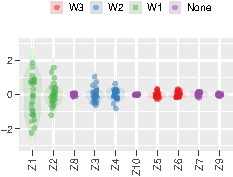
\includegraphics[width=0.45\linewidth]{main_files/figure-latex/simulated-data-1} }\subfloat[After Rotation\label{fig:simulated-data2}]{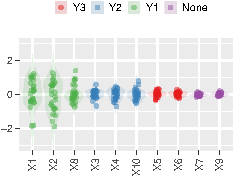
\includegraphics[width=0.45\linewidth]{main_files/figure-latex/simulated-data-2} }

}

\caption{Simulated Data before}\label{fig:simulated-data}
\end{figure}

Among several methods
\citep{anderson1987generation, heiberger1978algorithm} for generating
random orthogonal matrix, in this paper we are using orthogonal matrix
\(\mathcal{Q}\) obtained from QR-decomposition of a matrix filled with
standard normal variate. The rotation here can be a) restricted and b)
unrestricted. The latter rotates all components \(\mathbf{z}\) together
and makes all predictor variables somewhat relevant for all response
components. However, the former performs a block-wise rotation so that
it rotates certain selected predictor components together. This gives
control for specifying certain predictors as relevant for selected
responses, which was discussed in our example above. This also allows us
to simulate irrelevant predictors such as \(x_{7}\) and \(x_{9}\) which
can be detected during variable selection procedures.

\hypertarget{rotation-of-response-space}{\subsection{Rotation of
response space}\label{rotation-of-response-space}}

The previous example has four response variables with only three
informative components \(w_1, w_2\) and \(w_3\). During the rotation
procedure, the response space is also rotated along with the predictor
space. Figure \ref{fig:cov-plot-print} shows that the informative
response component \(w_3\) is rotated together with the uninformative
response component \(w_4\) so that the predictors which were relevant
for \(w_3\) will be relevant for response variables \(y_3\) and \(y_4\).
Similarly, response components \(w_1\) and \(w_2\) are rotated
separately so that predictors relevant for \(w_1\) and \(w_2\) will only
be relevant for \(y_1\) and \(y_2\) respectively, which we can see in
Figure\textasciitilde{}\ref{fig:simulated-data}. In the r-package
\emph{simrel-m}, the combining of the response components is specified
by a parameter \texttt{ypos}.

\hypertarget{implementation}{\section{Implementation}\label{implementation}}

This section demonstrates an application of multi-response extension of
\texttt{simrel} in order to compare different estimation methods on the
basis of prediction error. For the comparison, we have considered four
well established estimation methods.

\begin{enumerate}
\def\labelenumi{\alph{enumi})}
\tightlist
\item
  Ordinary Least Squares (OLS),
\item
  Principal Component Regression (PCR),
\item
  Partial Least Squares predicting individual response variable
  separately (PLS1) and
\item
  Partial Least Squares predicting all response variables together
  (PLS2).
\end{enumerate}

We have also considered four relatively new estimation methods in
multi-response regression:

\begin{enumerate}
\def\labelenumi{\alph{enumi})}
\tightlist
\item
  Canonically Powered Partial Least Squares regression (CPPLS)
  \citep{indahl2009canonical},
\item
  Canonical Partial Least Squares regression (CPLS)
  \citep{indahl2009canonical},
\item
  Envelope estimation in predictor space (Xenv)
  \citep{cook2010envelope},
\item
  Envelope estimation in response space (Yenv)
  \citep{cook2015foundations} and
\item
  Simultaneous estimation of x- and y-envelope (Senv)
  \citep{cook2015simultaneous}
\end{enumerate}

From the possible combinations of two levels of coefficient of
determination \((R^2)\) and two levels of \texttt{gamma} (the factor
that controls the multicollinearity in predictor variables), four
simulation designs (design 1-4) were prepared. Replicating each design
20 times, 80 datasets with five response variables \((m=5)\) and 16
predictor variables \((p = 16)\) were simulated using the method
discussed in this paper. It was also assumed that three principle
components of response variables (\(w_1, w_2\) and \(w_3\)) completely
describe the variation present in five response variables
(\(y_1 \ldots y_5\)). The four designs are presented in
Table\textasciitilde{}\ref{tab:parameter-settings}. All datasets
contained 100 sampled observations and out of 16 predictor variables,
three disjoint set of five predictor variables are relevant for response
components \(w_1, w_2\) and \(w_3\). Further, predictor components
\(z_1\) and \(z_6\) were relevant for response component \(w_1\),
predictor components \(z_2\) and \(z_5\) were relevant for response
component \(w_2\) and predictor component \(z_3\) and \(z_4\) was
relevant for response component \(w_3\). In addition, following the
discussion about \protect\hyperlink{rotation-of-response-space}{rotation
of response space}, \(w_1\) was rotated together with \(w_4\) and
\(w_2\) was rotated together with \(w_5\). Figure
\ref{fig:cov-plot-print-1} visualize the covariance structure and
relationship between the response and predictor variables for first
design.

\begin{figure}[!htb]
\subfloat[Relevant Position\label{fig:cov-plot-print-11}]{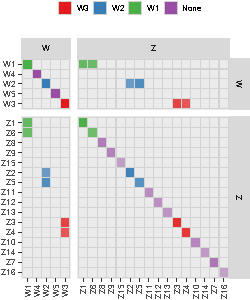
\includegraphics[width=0.33\linewidth]{main_files/figure-latex/cov-plot-print-1-1} }\subfloat[Rotation Matrix\label{fig:cov-plot-print-12}]{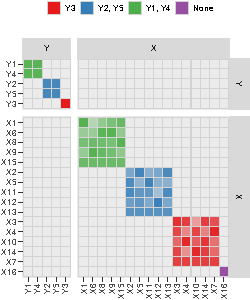
\includegraphics[width=0.33\linewidth]{main_files/figure-latex/cov-plot-print-1-2} }\subfloat[Relevant Predictors\label{fig:cov-plot-print-13}]{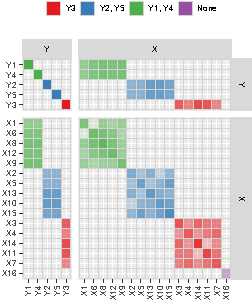
\includegraphics[width=0.33\linewidth]{main_files/figure-latex/cov-plot-print-1-3} }\caption{Simulation of predictor and response variables for design one after orthogonal transformation of predictor and response components by rotation matrices $Q$ and $R$ shown as the upper left and the lower right block matrices in (b).}\label{fig:cov-plot-print-1}
\end{figure}

\begin{table}[!h]

\caption{\label{tab:parameter-settings}Parameter setting of simulated data for comparison of estimation methods}
\centering
\begin{tabular}[t]{p{\dimexpr0.42\columnwidth-2\tabcolsep}p{\dimexpr0.14\columnwidth-2\tabcolsep}p{\dimexpr0.14\columnwidth-2\tabcolsep}p{\dimexpr0.14\columnwidth-2\tabcolsep}p{\dimexpr0.14\columnwidth-2\tabcolsep}}
\toprule
  & Design1 & Design2 & Design3 & Design4\\
\midrule
Decay of eigenvalues $(\gamma)$ & 0.2 & 0.8 & 0.2 & 0.8\\
Coef. of Determination $(\rho^2_{w_j})$ & 0.8, 0.8, 0.4 & 0.8, 0.8, 0.4 & 0.4, 0.4, 0.4 & 0.4, 0.4, 0.4\\
\bottomrule
\end{tabular}
\end{table}

For each method, an estimate of expected squared prediction error was
computed as,

\[\underset{m \times m}{\boldsymbol{\vartheta}} = 
\mathrm{E}\left[\left(
\hat{\boldsymbol{\beta}} - \boldsymbol{\beta}
\right) ^t \boldsymbol{\Sigma}_{xx}
\left(
\hat{\boldsymbol{\beta}} - \boldsymbol{\beta}
\right)\right] + \boldsymbol{\Sigma}_{y|x}\]

where, \(\hat{\boldsymbol{\beta}}\) is an estimate of true regression
coefficient \(\boldsymbol{\beta}\) and \(\boldsymbol{\Sigma}_{xx}\) is
the true covariance structure of the predictor variables obtained from
\texttt{simrel}. Also, \(\boldsymbol{\Sigma}_{y|x}\) is the true minimum
error of the model. Here \(\hat{\boldsymbol{\beta}}\) varies across
different estimation methods while the remaining terms are same for each
dataset design. Further, an overall prediction error of all responses is
measured by the trace of \(\boldsymbol{\vartheta}\).

The minimum prediction error (measured as discussed above) for nine
estimation methods averaged over 20 replications of four designs are
shown in Table \ref{tab:min-error}. The table also gives the number of
predictor components (response components in case of \texttt{Yenv}), a
method has used in order to obtain the minimum of average prediction
error.

\rowcolors{2}{gray!6}{white}

\begin{table}

\caption{\label{tab:min-error}Minimum average prediction error 
      (number of components corresponding to minimum prediction error, minimum prediction error) 
      (For $Y\text{env}$, the number of response components is given)}
\centering
\begin{tabular}[t]{>{\bfseries\raggedright\arraybackslash}p{7em}>{\ttfamily\centering\arraybackslash}p{6em}>{\ttfamily\centering\arraybackslash}p{6em}>{\ttfamily\centering\arraybackslash}p{6em}>{\ttfamily\centering\arraybackslash}p{6em}lcccclcccclcccclcccc}
\hiderowcolors
\toprule
\bfseries{Model} & \bfseries{Design: 1} & \bfseries{Design: 2} & \bfseries{Design: 3} & \bfseries{Design: 4}\\
\midrule
\showrowcolors
CPLS & (3, 3.24) & (4, 3.22) & (3, 4.09) & (3, 4.05)\\
CPPLS & (3, 3.21) & (3, 3.17) & (3, 4.11) & (3, 4.04)\\
OLS & (1, 3.60) & (1, 3.58) & (1, 4.57) & (1, 4.50)\\
PCR & (7, 3.28) & (6, 3.19) & (6, 4.08) & (6, 4.04)\\
PLS1 & (2, 3.32) & (5, 3.20) & (1, 4.16) & (5, 4.07)\\
\addlinespace
PLS2 & (5, 3.29) & (6, 3.19) & (3, 4.11) & (6, 4.06)\\
Senv & (4, 3.17) & (5, 3.14) & (3, 4.35) & (5, 4.28)\\
Xenv & (5, 3.23) & (6, 3.20) & (5, 4.10) & (6, 4.11)\\
Yenv & (3, 3.24) & (3, 3.23) & (3, 4.29) & (3, 4.24)\\
\bottomrule
\end{tabular}
\end{table}

\rowcolors{2}{white}{white}

Table \ref{tab:min-error} shows that the simultaneous envelope has
prediction error of 3.17 and 3.14 in design 1 (with 4 components) and
design 2 (with 5 components), respectively, which is smaller than other
methods. However the method was not able to show the same performance in
design 3 and design 4. The PCR model has the smallest prediction error
(4.08) from 6 components in design 3 and Canonically Powered PLS has
minimum prediction error (4.04) from 3 components in design 4. In design
3, we can also see that the Canonical PLS method has second best
performance with only three components. The number of components vary
across different replicated dataset but the component corresponding to
minimum prediction error is discussed here. A detailed picture of
prediction error for each estimation method obtained for each additional
component is shown in Figure \ref{fig:Average-Prediction-Plot}. Although
designs 2 and 4 have higher levels of multicollinearity, the performance
of the estimation methods is indifferent to its effect. Since all the
methods, except OLS, are based on shrinking of estimates, they are less
influenced by the multicollinearity problem.

\begin{figure}[!htb]
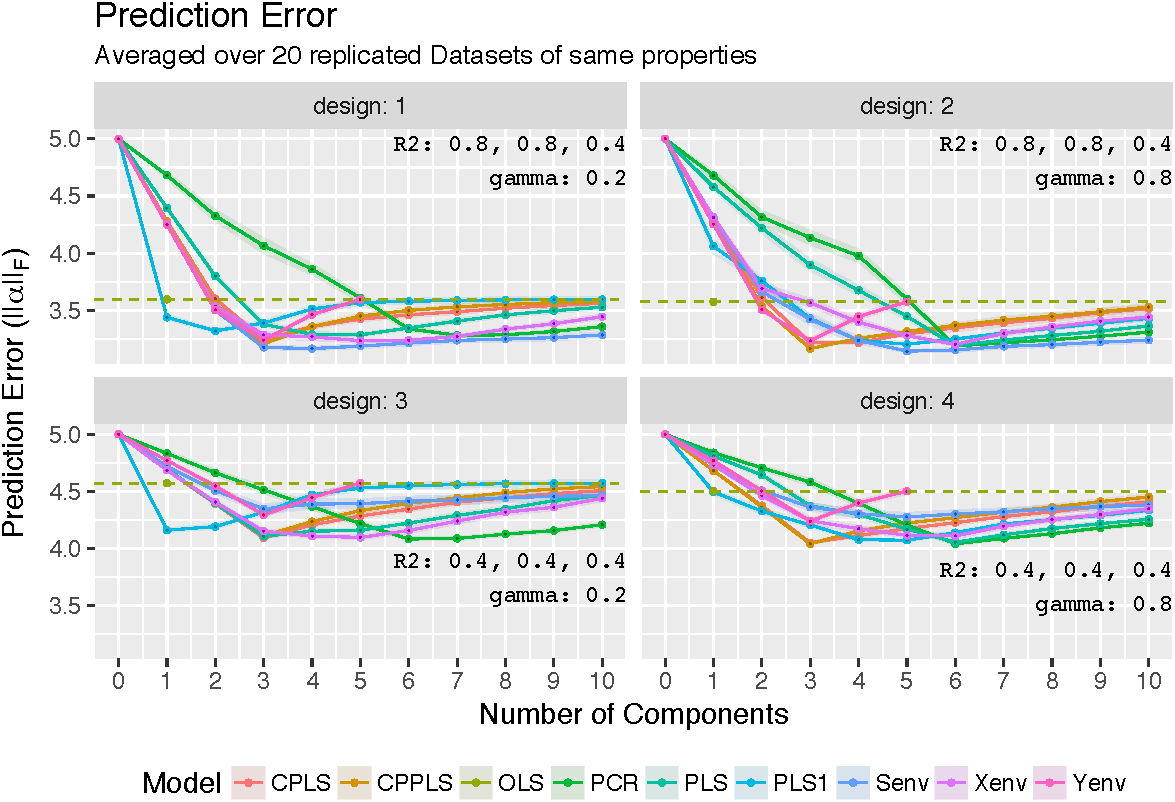
\includegraphics[width=1\linewidth]{main_files/figure-latex/Average-Prediction-Plot-1} \caption{Minimum of Average Prediction Error}\label{fig:Average-Prediction-Plot}
\end{figure}

The analysis presented in Figure \ref{fig:Average-Prediction-Plot} has
addressed some questions such as how methods work when there exist a
true reduced dimension in response space, but also arose other questions
like why they perform differently. For example, what is the reason for
the decreasing relative performance of the simultaneous envelope method
as the \(\rho^2\) values are reduced? Does this depend on the dimensions
and shape of the \(\mathbf{y}\) envelopes? Since, the example is merely
intended as a demonstration of how \texttt{simrel} can be used in
scientific study, a more elaborative studies would be necessary to
answer such questions, but for this purpose \texttt{simrel} would be a
powerful tool.

\section{Web Interface}\label{web-interface}

In order to give an alternative interface for \texttt{simrel}, we have
created a shiny app which allows users to input the simulation
parameters through different input fields. Figure \ref{fig:AppSimulatr}
shows a screenshot of the application. The application contains three
main sections through which the user can interact with this simulation
approach. A random seed can be selected using section Figure
\ref{fig:AppSimulatr} (a) so that a particular set of data can be
re-simulated if needed. Figure \ref{fig:AppSimulatr} (b) has all the
input panels where the user dependent parameters for simulation can be
entered. Here the user also has the option to simulate univariate (uses
\texttt{simrel} package in CRAN), bivariate (not yet available in CRAN)
and multivariate simulation (\texttt{simrel-m}). In addition, a
simulated R-object comprised by the simulated data can be download as
\texttt{Rdata} format (section (e) in Figure \ref{fig:AppSimulatr}). The
object holds the simulated data along with other properties such as
coefficient of determination for each response, true regression
coefficients and rotation matrices.

All \texttt{simrel} parameters can be entered using a simple user
interface where a vectors are separated with comma(,) and lists are
separated with semicolon(;). For instance, the relevant position
discussed in the \protect\hyperlink{implementation}{implementation}
section of this paper can be entered as \texttt{1,\ 6;\ 2,\ 5;\ 3,\ 4}
which is equivalent to R syntax
\texttt{list(c(1,\ 6),\ c(2,\ 5),\ c(3,\ 4))}.

\begin{figure}[!htb]

{\centering 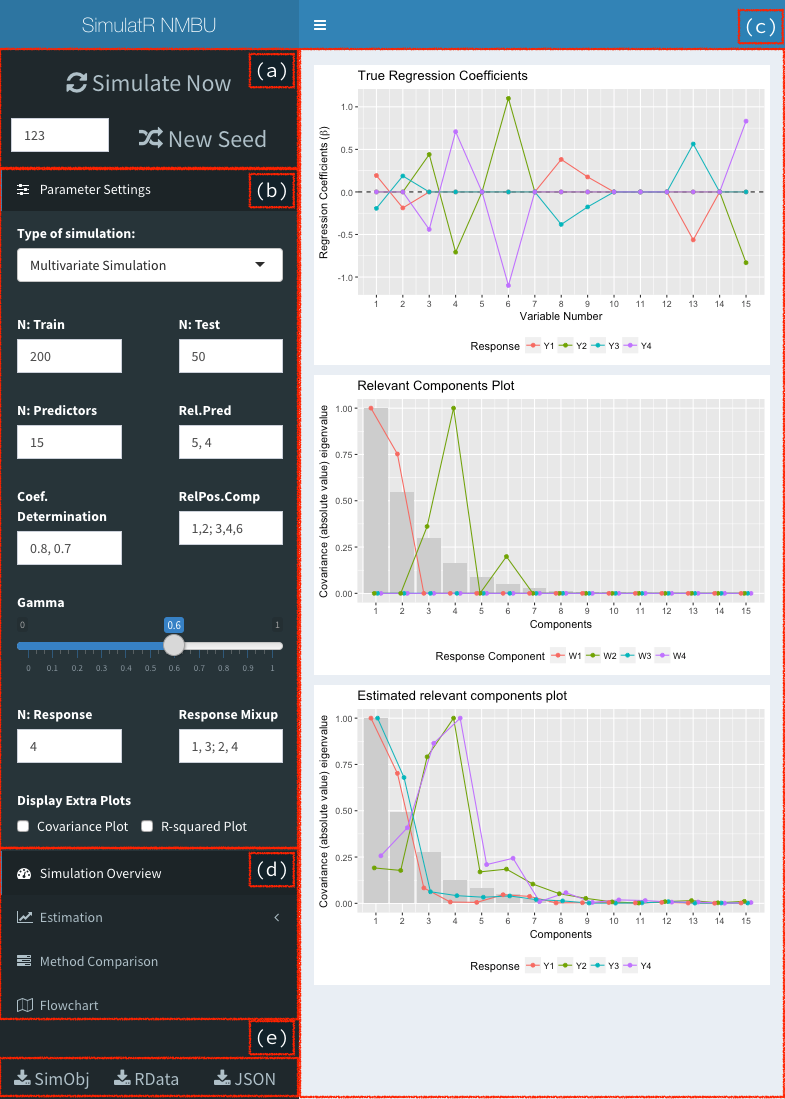
\includegraphics[width=0.95\linewidth]{images/AppSimulatr} 

}

\caption{Application interface of `simulatr`. (a) Seed and simulation button (b) Parameter control panel (c) Properties of simulated data (d) Additional analysis (e) Download option of simulated data}\label{fig:AppSimulatr}
\end{figure}

The application not only allows users to simulate data, but also gives
some insight into simulated data properties. The example used in the
screenshot has simulated 200 training and 50 test samples with 15
predictor and 4 response variables. There are two latent variables
(response components) that completely span the informative response
space. Five predictor variables are relevant for the first response
component and explains 80 percent of the variation in \(\mathbf{x}\). In
addition, the first and second predictor components span the same space
as spanned by these five relevant predictors. Similarly, another set of
four predictor variables are relevant for second response component and
explains 70 percent of the variation. Here, third, fourth and sixth
predictor components span the same space as spanned by these four
relevant predictors. Further, the first response component is rotated
together with a normally distributed random vector to obtain first and
third response variable and second response components are rotated
together with another normally distributed random vector to obtain
second and fourth response variable.

Section (c) in Figure \ref{fig:AppSimulatr} contains three plots -- a)
true regression coefficients b) relevant components and c) estimated
relevant components. In the first plot we can see that predictor
variables (1, 2, 8, 9 and 13) are relevant for the first and third
response variable by their non-zero coefficients, whereas predictor
variables (3, 4, 6 and 15) are relevant for the second and fourth
response variable. The second plot shows the covariances between the
response components and the predictor components along with the
corresponding eigenvalues in the background (bar plot). In the plot the
absolute value of the covariances after scaling with the largest
covariance are shown. As in our parameter setting, the plot shows that
first and second predictor components have non-zero covariance with
first response component and third, fourth and sixth predictor
components have non-zero covariance with second response component. The
third plot is the estimated covariance between predictor components and
the response variables, for the simulated data. Since the first and
third response components are rotated together, in the plot, the
covariance between predictor components and first and third response
variable is following similar pattern. This also suggests that the
predictor components which were relevant for first response components
gets relevant for first and third response variables after rotation.

Along with these main sections, section (d) in the figure contains
additional analysis performed with the simulated data such as its
estimation with different methods. This section is intended for
educational purposes to show how changing the data properties influences
the performances of different estimation and prediction methods.

Many scientific studies
\citep{helland2012near, saebo2008lpls, cook2015simultaneous} are using
simulated data in order to compare their findings with others or assess
its properties. In many of these situations, a user-friendly and
versatile simulation tool like \texttt{simrel} can play an important
role. \citet{gangsei2016theoretical} and \citet{saebo2015simrel} are
some examples where the univariate and bivariate form of \texttt{simrel}
have been used for such purposes.

\section{References}\label{references}


\renewcommand\refname{References}
\bibliography{packages.bib,ref-db.bib}


\end{document}
